% This is ''sig-alternate.tex'' V2.0 May 2012
% This file should be compiled with V2.5 of '\'sig-alternate.cls'' May 2012
%
% This example file demonstrates the use of the \'sig-alternate.cls'
% V2.5 LaTeX2e document class file. It is for those submitting
% articles to ACM Conference Proceedings WHO DO NOT WISH TO
% STRICTLY ADHERE TO THE SIGS (PUBS-BOARD-ENDORSED) STYLE.
% The \'sig-alternate.cls' file will produce a similar-looking,
% albeit, 'tighter' paper resulting in, invariably, fewer pages.

\documentclass{sig-alternate}
\sloppy
\usepackage{paralist}
\usepackage{url}
\usepackage[pdftex]{hyperref}

\begin{document}
%
% --- Author Metadata here ---
\conferenceinfo{SIGCSE}{2016 Memphis, Tennessee, USA}
\CopyrightYear{2016} % Allows default copyright year (20XX) to be over-ridden - IF NEED BE.
%\crdata{0-12345-67-8/90/01}  % Allows default copyright data (0-89791-88-6/97/05) to be over-ridden - IF NEED BE.
% --- End of Author Metadata ---


% Original title: Ailfeddwl Cyfrifiadureg yn Ysgolion Cymru\\(or: Rethinking Computer Science in Welsh Schools)

\title{On the Need and Impact of Technocamps\\on Computing Education in Wales}

 \numberofauthors{2}
% \author{
% % 1st. author
% \alignauthor
% Tom Crick\\
% \affaddr{Department of Computing}\\
% \affaddr{Cardiff Metropolitan University, UK}\\
% \affaddr{tcrick@cardiffmet.ac.uk}
% % 2nd. author
% \alignauthor
% Faron Moller\\
% \affaddr{Department of Computer Science}\\
% \affaddr{Swansea University, UK}\\
% \affaddr{f.g.moller@swansea.ac.uk}\\
% }

\maketitle

\begin{abstract}
Computer science education in the United Kingdom has undergone
substantial scrutiny, and in England a new computing curriculum has
just been introduced.  However, in Wales -- a devolved nation in the
UK -- political, geographical and socio-technical issues hinder any
substantive educational policy or curriculum reform for computer
science.  In this paper we outline the impact of Technocamps, a
university-based schools outreach programme founded in 2003.
\end{abstract}

% A category with the (minimum) three required fields
\category{K.3.2}{Computers \& Education}{Computer and Information Science Education}[Computer Science Education]
\category{K.4.1}{Computers And Society}{Public Policy Issues}
\keywords{Computer Science Education; High School; Teachers;
  Professional Development, Policy, Wales, UK}

% preamble -- a note on UK terminology?


\section{Introduction}\label{intro}

%\section{Computing Education in the UK}\label{compedu}

In the 1980s, computer studies was a popular subject in schools across
the UK. As mentioned previously, the ubiquitous presence, in both
schools and homes, of the popular BBC Micro -- which was useful for
little else unless you were able to program -- saw a large proportion
of school children learning the fundamentals of programming in a
curriculum which included a variety of complementary topics such as
hardware, software, Boolean logic and binary number
representation.
% ~\cite{Doyle:1988}

% In the early 1980s, the BBC Micro was introduced to schools throughout
% the UK as part of the BBC's \emph{Computer Literacy Project}; before
% long they were in 80\% of UK classrooms~\cite{vasko:1986}. By
% encouraging young learners to experiment with computers, a generation
% of creative (and computational) talent was spawned. Applications in
% the UK to study computer science at university hit a peak, with
% computer science graduates helping computers come to dominate every
% aspect of our lives.

By the 1990s, however, the emergence of pre-installed software
packages -- specifically office productivity software such as word
processors and spreadsheet programs -- meant that computers were no
longer predominantly machines that needed to be programmed in order to
do anything useful or interesting.  Less and less time was being spent
in the computer studies classroom on thinking about and writing
programs, as basic digital literacies and IT skills became regarded as
the priority. However, as interest in viewing the computer as a
creative tool waned in favour of using it for more mundane tasks,
various problems were being created, which were highlighted in two
independent enquiries in 1997: the McKinsey
Report~\cite{McKinsey:1997} and the Stevenson
Report~\cite{Stevenson:1997}.  Both reports concluded that Information
Technology in UK schools was in a primitive state and in need of
attention and major investment. In line with the Stevenson Report,
computer studies evolved into a new subject whose name was coined in
that same report: {\emph{Information and Communications Technology}}
(ICT).  Over the decade starting in 1997, the UK Government invested
over \pounds3.5 billion in ICT in schools through various initiatives
such as the National Grid for Learning (NGfL) and the New
Opportunities Fund (NOF)~\cite{Doughty:2006}.

By 2000, then, ICT had permeated both primary and secondary school
curricula, not least in the newly-devolved nations. The emphasis was
on developing the children's IT skills and digital literacy in an
honest attempt to address the increasing need for digital competencies
amongst the general public.  However, despite enormous
government-funded ICT initiatives, various reports throughout the
decade identified problems with implementing government policy on ICT
educational
reform~\cite{OpieFukuyo:2000,Ofsted:2001,Ofsted:2002,Ofsted:2004,
Loveless:2005}. Younie~\cite{Younie:2006} summarises the problems
identified by these reports into five key areas, three being
management and the other two being: teacher training and competence;
and impact on pedagogy.  The ICT curriculum in
Wales~\cite{welshictcurric:2008}, while generally viewed to be more
flexible and less prescriptive than the equivalent subject in England,
exhibited many of the same
issues~\cite{estynict:2007,estynict:2013,estynict:2014}. A full
two-thirds of ICT teachers in the UK do not have a relevant
qualification but may have moved into the role of ICT teacher simply
by being sufficiently digitally literate~\cite{RoyalSoc:2012}.  The
situation is worse in Wales, where this figure rises to
75\%~\cite{GTCW:2008}, with ICT perceived to be a low-priority
discipline in schools. Applications to study computer science at
university slumped in the early part of the millennium -- especially
amongst females -- and many of those who started a university computer
science degree course found themselves dropping out during the first
year, surprised at what computer science is and what studying it
entails.

% Nesta Next Gen.?
A decade later, a report by the Royal Society~\cite{RoyalSoc:2012},
the UK's premier science academy, made the very same observations.
The report noted that ICT suffers from a poor reputation amongst
pupils, parents and industry, who consider it dull and unchallenging
and hence a low-value discipline, especially compared to other
strategically-significant STEM subjects.  With ICT embedded across the
primary school curriculum, secondary school pupils find ICT in
secondary school neither stimulating nor engaging. The Wolf
Report~\cite{Wolf:2011} further notes that the undemanding nature of
ICT qualifications in secondary schools is readily exploited by schools:
due to a high league table weighting associated with
vocational qualifications, easily-achieved high results in ICT offer a
welcome boost to a school's league table position. Furthermore, as ICT
is typically presented by schools as their ``computing'' offering,
students who might otherwise enjoy studying computer science are
actively put-off from what they are wrongly but innocently
led to believe is computer
science~\cite{crick+sentance:2011,brown-et-al-sigcse2012}.

% Fast forward 30 years and the situation is very much different. The
% computer is no longer a novelty; children now typically spend more
% time in front of a computer screen than a TV screen at home, but like
% the TV, their interest is restricted to using the computer, not in
% experimenting with it. Computer studies in school -- since the late
% 1990s generally named Information and Communications Technology (ICT)
% -- has evolved into IT studies with an emphasis on digital literacy
% and ``office productivity'' skills -- significantly more mundane than
% the social networking and gaming for which many pupils use their
% personal digital devices. A full two-thirds of ICT teachers in the UK
% do not have a relevant qualification but may have moved into the role
% of ICT teacher simply by being sufficiently digitally
% literate~\cite{RoyalSoc:2012}.  The situation is worse in Wales, where
% this figure rises to 75\%~\cite{GTCW:2008}, with ICT perceived to be a
% low-priority discipline in schools. Applications to study computer
% science at university slumped in the early part of the millennium --
% especially amongst females -- and many of those who started a
% university computer science degree course found themselves dropping
% out during the first year, surprised at what computer science is and
% what studying it entails.

% Recognising this trend, the Department of Computer Science at Swansea
% University in the early 2000s started looking into ways to address
% this issue.  Unfortunately, attempts to reach out to teachers in local
% schools faced great resistance, in part due to their lack of
% confidence in teaching actual computer science as opposed to
% developing skills in using specific desktop software packages.

% As an alternative route to effecting change and getting into schools,
% Swansea University created
% Technocamps\footnote{\url{http://www.technocamps.com}} in 2003, an
% outreach programme to bring groups of school children to the
% university campus for day-long workshops based on selected
% computational themes to inform them what computing is about,
% followed-up by support in setting up extracurricular clubs --
% \emph{Technoclubs} -- in the schools.  Technocamps proved hugely
% successful as a local initiative, with many students opting to study
% computer science at Swansea University claiming to be influenced by
% Technocamps activities.

% In 2010, based on long-term empirical data regarding its effect on
% school children's attitudes towards computer science and technology
% careers -- as well as their teachers' -- Swansea University was
% awarded \pounds 3.9 million funding towards a \pounds 6 million
% four-year project (with the remaining \pounds 2.1 million generated
% through matched funding from the university) by the Welsh Government
% under the EU's European Social Fund (ESF) Convergence
% Programme\footnote{\url{http://wefo.wales.gov.uk/programmes/20072013/convergence/?lang=en}}
% to run Technocamps as a pan-Wales project with regional hubs at the
% Universities of Aberystwyth, Bangor and Glamorgan (now University of
% South Wales)\footnote{As discussed in further detail in
% Section~\ref{technocamps}, Technocamps hubs have subsequently been set
% up at most of the remaining major Universities in Wales, specifically
% Cardiff University, Cardiff Metropolitan University, and Glynd\^wr
% University in Wrexham.}  Though focusing on the children, Technocamps
% also provides ``Technoteach'' events aimed at up-skilling ICT teachers
% in Wales.  Technocamps has since provided computer science-related
% activities and resources for tens of thousands of young people across
% Wales, as well as interacting with hundreds of teachers across
% hundreds of the nation's schools.

% Technocamps is not alone in exploring solutions to the multitude of
% problems in computer science education in the UK.  In particular, in
% 2008 the Computing At School
% (CAS)\footnote{\url{http://www.computingatschool.org.uk}} organisation
% was formed, which has since been recognised as the UK subject
% association for computer science and a key stakeholder from a policy
% perspective. Its current membership of over 18,000 teachers and
% computing professionals work hard to promote the teaching of computer
% science at school. However, whilst great changes have taken place in
% England due in no small part to CAS lobbying and on the ground
% initiatives\footnote{Its contributions to the new Computing curriculum
% in England were recognised by winning the 2014 Informatics Europe Best
% Practices in Education
% Award: \url{http://www.computingatschool.org.uk/index.php?id=best-practice-in-education-award-2014}}
% -- underpinned by generous funding of CAS by England's Department of
% Education -- the wider CAS effect has been less noticeable in Wales,
% with the rapid curriculum changes pushed through in England in many
% ways resisted by the Welsh Government.

% Wales is one of the four devolved nations within the UK, with its own
% elected national government fully responsible for its education
% system.  In 2012, the Welsh Government's Minister for Education and
% Skills publicly acknowledged the importance of computer science
% education for all -- noting the impact of Technocamps -- and expressed
% understanding of the wider educational and socio-economic impact that
% the government can make with educational reform in Wales.  However,
% with only 5\% of the population of England and with its distinct
% geographical and socio-cultural challenges, Wales presents a variety
% of unique challenges in addressing curriculum reform. Nevertheless,
% since 2013 we have seen significant industry and public scrutiny of
% the relevancy of the school curriculum and the changing skills demands
% of the wider digital economy, with a range of government-initiated
% independent reviews of ICT culminating in a substantial review of the
% wider national curriculum. Wales is thus on the cusp of substantial
% reform, with Technocamps and CAS having a front-line role in the
% development of a new computing curriculum, as well as supporting the
% professional development of teachers.

Technocamps, a Welsh university-based schools outreach programme,
was founded in 2003 to address these emerging problems,
and its portfolio of activities is outlined in~\cite{crick+moller-wipsce2015}.
In this paper, we consider the need and the impact that Technocamps has had,
evidencing this through the consideration of its measurable effect
on schools, teachers, and education policy changes in Wales.

\section{Devolved Education in the UK}\label{welshukedu}

%The UK consists of four nations ruled by one parliament, with an
%overall population of 64.1 million: England (population: 53.9
%million), Scotland (5.3 million), Wales (3.1 million) and Northern
%Ireland (1.8 million)~\cite{onspop:2014}. In 1997, Scotland and Wales
%held referendums which determined in both cases the desire for
%self-government.  In the case of Wales, this led to the Government of
%Wales Act 1998 which created the National Assembly for Wales, to which
%a variety of powers were devolved from the UK parliament on 1 July
%1999 (and again with the Wales Act 2014).  In particular, education --
%which until then was a UK-wide government portfolio (minus Scotland,
%which for historical reasons has had a distinct legal and education
%system from England and Wales) -- came under the control of the
%National Assembly for Wales, under the direction of the Department for
%Education and Skills (originally the Department for Children,
%Education, Lifelong Learning and Skills).

Wales is a small nation to the west of England with an ancient
Celtic culture and a thriving language (with c.20\% of the population
able to speak Welsh).  Its south coast became pre-eminent during the
Industrial Revolution due to coal mining and heavy industry; however,
Wales is mostly rural and suffers from post-industrial poverty,
seasonal employment and the dependence on the public sector for a
significant proportion of jobs. The country is sparsely populated with
resilience and interconnectedness of the transport infrastructure an issue.
Hence its communities -- and more specifically its schools and
teachers -- suffer from the perils of isolation. Apart from the south
east corner (including its capital Cardiff)
and the regions bordering England, the rest of the country
is formally designated by the EU as a so-called ``Convergence area'',
meaning its per-capita gross domestic product (GDP) is less than 75\%
of the EU average.

Politically, Wales became a devolved nation within the UK in 1999.
Prior to devolution, the education system in Wales was essentially
identical to that in England and was in a healthy state, outperforming
other regions in the UK in the years prior to and immediately
following devolution.  However, since devolution saw the education
portfolio transferred to the National Assembly of Wales, it has
suffered a rapid decline. Evans~\cite{Evans:2015} carries out a
detailed analysis as to why this was the case, citing a multitude of
policy changes and poor interventions, alongside a hard-hitting report
from the OECD~\cite{oecdwales:2014}.

% \begin{figure*}[htp]
% \centering
% \begin{picture}(445,250)(-5,-55)
% %\put(-5,-55){\framebox(445,250){}}
% \put(10,0){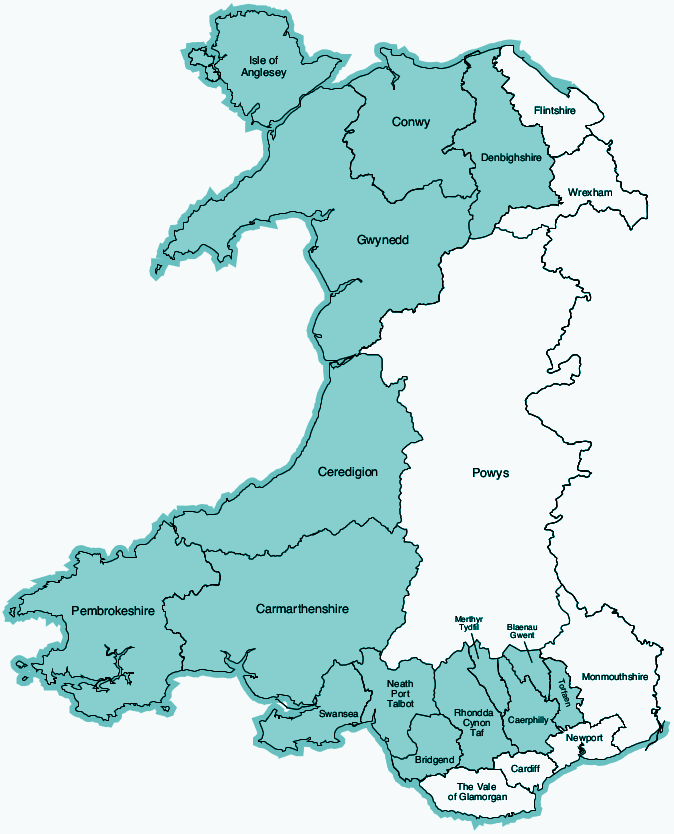
\includegraphics[width=0.31\textwidth]{images/wales.png}}
% \put(275,0){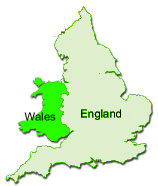
\includegraphics[width=0.325\textwidth]{images/UK.png}}
% \put(165,96){\line(6,-1){128}}
% \put(10,1){\dashbox(155,190){}}
% \put(293,45){\dashbox(58,68){}}
% \put(90,-35){\makebox(0,0){\begin{tabular}[t]{@{\hspace{1em}}r@{ }l}
% (a) & Convergence area of Wales, which \\ & encompasses 15 (out
% of 22) western \\ & councils that do \emph{not} border England
% \end{tabular}}}
% \put(360,-20){\makebox(0,0){(b)~Wales and England}}
% \end{picture}
% \caption{Maps of Wales and England}
% \label{fig:wales}
% \end{figure*}

% \begin{figure}[!ht]
%   \centering
%   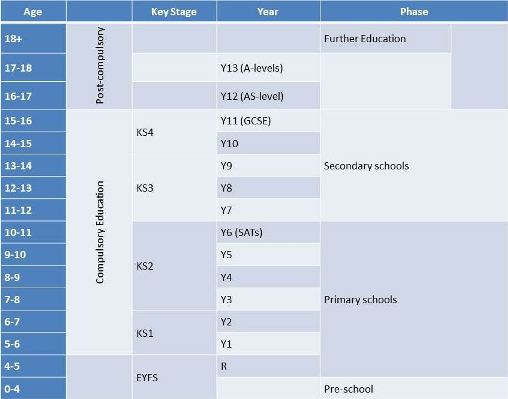
\includegraphics[width=0.9\columnwidth]{images/keystages.png}
%   \caption{Key Stages in the English and Welsh education system}
%   \label{fig:key-stages}
% \end{figure}

% \begin{itemize}
% \item phasing out national Standard Attainment Tests (SATs);
% \item replacing the early years Key Stage 1 with a learning through
% play-based Foundation Phase;
% \item introducing the Welsh
% Baccalaureate\footnote{\url{http://www.welshbaccalaureate.org.uk/}} at
% all levels: an overarching qualification, with a purely
% practical-based assessment mechanism, incorporating key skills; Wales,
% Europe and the world; work-related education; and personal and social
% education;
% \item emphasising the focus on the Welsh language and Welsh-medium
% schools;
% \item addressing the abundance of small schools in the predominantly
% rural communities throughout Wales;
% \item tackling deprivation.
% \end{itemize}

Whilst broadly maintaining the general educational system
used in England, the Welsh
Government embarked on a 10-year revolutionary plan including
%phasing out national Standard Attainment Tests (SATs),
introducing the Welsh
Baccalaureate %\footnote{\url{http://www.welshbaccalaureate.org.uk/}}
(an overarching qualification, with a purely practical-based
assessment mechanism, incorporating key skills) as well as explicitly
using education as a lever to tackle socio-economic deprivation.
Much of this plan was lauded, being learner-focused, placing an
emphasis on skills development and ensuring that it is appropriate for
the specific needs of Wales. However, since its implementation, it has
been criticised for various reasons and by various stakeholders.  The
then Minister for Education and Skills appointed in June 2010, in
looking for the causes of Wales' failing education system, found cause
to commission no fewer than 24 costly reviews before his untimely
resignation in February 2013 -- almost one per
month~\cite{Evans:2015}.

With devolved government comes autonomy over fiscal matters; and the
correlation between money and performance is an obvious target for
critics, who point to a growing spending shortfall between Wales and
England.  The average spend per pupil in Wales in 2000-2001 -- just
after devolution -- was more than every region of England apart from
the large metropolitan areas of London, the West Midlands and the
North West, all of which benefit from their vast economies of scale.
However, since then, the gap between the education budgets per pupil
between Wales and England has steadily grown by about 1\% per year.
%the figures forecast for 2013-2014 show 13\% more being spent per
%pupil in England than in Wales (\pounds7,533 per pupil in England as
%opposed to \pounds6,676 per pupil in Wales)~\cite{Evans:2015}.

%As reported by Hubweiser et al.~\cite{hubwieser-et-al:2011}, when
%establishing a model for viewing school computer science education, it
%is apparent that there is much diversity between school education
%systems, and this can create an obstacle when trying to understand
%progress made in a different country; this is particularly pertinent
%to the devolved educational systems of the UK.

%\section{Technocamps}\label{technocamps}

%\subsection{Technocamps and Swansea University}\label{techoswansea}

% As experienced by other UK universities, the numbers of students
% enrolling in computer science degree programmes at Swansea University
% increased through the end of the millennium due to the dot-com boom.
% However, as depicted in Figure~\ref{fig:numbers},
% \begin{figure}%[!ht]
%   \centering
%   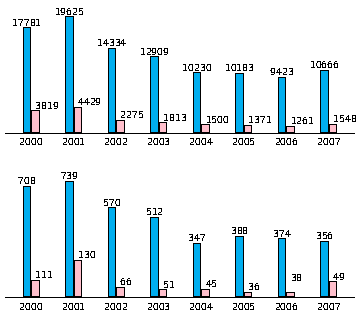
\includegraphics[width=0.9\columnwidth]{images/numbers.png}
%   \caption{Applications to University computer science degree programmes
%            in the UK (top) and Wales (bottom), males (blue) and females (pink).
%            (source: Universities and Colleges Admissions Service
%            (UCAS))}
%   \label{fig:numbers}
% \end{figure}
% throughout the UK
% (as elsewhere) the numbers then peaked, and what followed was a steady
% five-year decline, dropping more than 40\% during that period, with
% the worst effect on the already-dwindling numbers of female students.
% Even at its peak, more than a third of students who started a computer
% science degree programme left the programme before their second year
% of study, citing a mistaken understanding of the subject as their
% primary reason for leaving
% (in line with the findings in~\cite{brown-et-al-toce2014}).

% In an attempt to address this worrying anomaly, the Department of
% Computer Science at
% Swansea\footnote{\url{http://www.swansea.ac.uk/compsci}} reached out
% to local secondary school ICT teachers, inviting them to meetings at
% the university, and offering to visit schools to discuss the subject
% with the teachers and to give motivational talks to students. Indeed,
% the Department was invited every year to a number of schools in
% England to present such talks to school children making their
% university admissions selections.  However, interest locally was more
% than absent: there was positive resistance to the department giving
% talks to their prospective university applicants; such activity was
% typically characterised as merely nakedly ``pitching for students.''
% In reality, for reasons explained later which did not apply to
% teachers in England, teachers in Wales were generally feeling
% over-burdened and disinterested in exploring any perceptions of
% inadequacy in the curriculum and their
% delivery~\cite{crick+sentance:2011,boyle-et-al:2012,brown-et-al-toce2014,crick+moller-wipsce2015}.

% As it appeared to be futile to influence schools and their ICT
% teachers directly, Technocamps was created in 2003 to promote
% computing amongst their pupils.  This was a programme of engaging
% interactive computational workshops taking place on the university
% campus whose ultimate aim was to subtly re-introduce computer science
% into the ICT curriculum by generating the demand from the students.
% Originally run only at Swansea University, Technocamps hubs have since
% been created at most universities throughout Wales, offering wide
% geographical coverage.

% Teachers in Wales were happy to ``treat'' their classes to these ``day
% out'' activities; but they were then faced with the prospect of
% satisfying their pupils' newly-discovered passion for computing,
% programming and computational thinking by introducing ``Technoclubs''
% as lunch-time extra-curricular activities in the school.  With
% generous help, resources and guidance from Technocamps -- along with
% the fact that in many cases students appeared to be more technically
% informed and digitally literate than their
% teachers~\cite{sentance-et-al-wipsce2012} -- these clubs have
% flourished, and the impact of Technocamps in changing attitudes in
% Welsh schools regarding ICT and computing has been widely
% acknowledged, both by the Welsh Government and National Assembly for
% Wales, as well as the teaching community in Wales.
% %%( This appears later on)
% %An independent
% %review of Technocamps activity in the (socio-economically
% %disadvantaged) Convergence area of Wales carried out for Welsh
% %Government estimates that 5\% of Welsh secondary students (ie, aged
% %11-19) have engaged with Technocamps through Workshops, and that more
% %than a quarter of the secondary schools in the region have established
% %Technoclubs~\cite{Wavehill:2015}.

% \subsection{The Technocamps Programme}\label{technoprogramme}

% As indicated above, Wales provides a variety of major challenges --
% political, geographical, socio-economic -- in reforming its curriculum
% to re-introduce computer science into the space currently populated by
% ICT, with its preponderance of IT skills development.  Whilst there is
% clear industrial support for educational reform which notes the
% importance of high-value digital skills for long-term economic renewal
% for Wales as an agile ``digital economy'', there has been relatively
% little interest in this amongst schools, teachers and politicians.
% Thus, any attempt at stimulating change would require significant
% resources and infrastructural investment.

% Technocamps was created to take up this challenge, through a
% multi-faceted university-based operation engaging with schools,
% interacting with both pupils and their teachers throughout Wales and
% across all ages. Its main activities are as follows:

% \begin{description}
% \item[Workshops]
% One-day campus-based workshops offered to whole classes
% to give the pupils an introduction to computing,
% particularly computational thinking and real world problem solving.
% The whole class approach allows us: to address the gender divide,
% by engaging with an equal number of boys and girls;
% and to engage with those with no predisposition (or indeed a clear aversion)
% to digital technologies, creating an interest in computing and its
% application to the world~\cite{ball-et-al:2012}.
% \item[Technoclubs\footnotemark]\footnotetext{\url{http://www.technocamps.com/technoclubs}}
% Lunchtime clubs in schools where pupils develop
% their computational thinking and building skills.
% \item[Bootcamps]
% Two-day campus-based workshops held during school holidays.
% \item[After Schools Clubs]
% Two-hour late afternoon sessions held on campus or in the community.
% There are two types of such clubs: one standard computing club
% in which participants get lessons, tutoring and individual help
% on all manner of programming tasks, for example with Python, Visual
% Basic, XHTML/CSS,  RobotC or an Arduino robotics project;
% and the other on computational thinking, called the Logic Club,
% in which the participants work on problem-solving tasks,
% typically developing step-by-step algorithmic solutions
% to a series of problems of varying difficulty.
% \item[Playground Computing\footnotemark]\footnotetext{\url{http://www.playgroundcomputing.com}}
% Day-long school-based workshops which present
% the fundamentals of computer science to primary school pupils
% through playful activities which develop computational thinking
% and problem solving skills, but do not involve computers.
% \item[Technoteach\footnotemark]\footnotetext{\url{http://www.technocamps.com/technoteach}}
% Training sessions, typically in the form of 20-hour modules
% delivered one evening per week over six weeks.
% The Technoteach modules have been accredited by ASFI
% -- Accredited Skills For Industry --
% for their Certificate in Computing for Teaching.
% Technoteach also encompasses other standalone twilight sessions
% as well as an annual teachers conference.
% \item[NEET Engagement]
% Week-long Summer residential sessions run in partnership with
% the municipal youth services in which young people identified
% as NEET (``Not in Employment, Education or Training'')
% carry out a variety of team-building exercises,
% learn app development and compete to design and build the best app.
% \item[Student Placements]
% Computer Science students at the university are offered
% the opportunity to gain credits for their university degree programme through
% placements -- one day per week -- as teaching assistants
% in school computing/ICT classes.
% \end{description}

% A key factor in the success of Technocamps has been that all
% Technocamps activities are provided completely free of charge for all
% of its participants. While this represents a significant investment on
% the part of the university partners, Technocamps has also received
% various sources of funding in support of its activities; the main
% funders are as follows:

% \begin{description}
% \item[European Social Funds] (October 2010 - September 2014) --
% A four-year \pounds 6 million Welsh Government/EU-funded project to
% engage with secondary schools across South West Wales and the
% Valleys. This project involved Technocamps hubs at Aberystwyth
% University, Bangor University and University of Glamorgan (now the
% University of South Wales). Some 9,000 pupils from more than 180
% schools and colleges have benefited from this project, as well as
% their teachers.

% \item[Nesta] (June 2013 - December 2014) --
% An 18-month \pounds 46,000 project to support the Playground Computing
% programme. This funding allows for a teacher to be seconded for 18
% months to Technocamps in order to go out to primary schools throughout
% South Wales every day to present workshops. It has seen some 5,000
% pupils at over 50 primary schools enjoy multiple day-long visits.

% \item[National Science Academy, Welsh Government] (November 2013 - March 2015) --
% A 17-month \pounds 24,000 project to support the Technoteach programme
% by the Welsh Government's NSA Grant Scheme; this funding was mainly in
% support of teachers registering on our six-week Technoteach modules,
% specifically providing their schools an amount of teacher cover to
% facilitate their attendance on the module. Over 120 teachers have thus
% far benefited from this project.

% \item[Learning in Digital Wales, Welsh Government] (September 2014 - March 2016) --
% An 18-month \pounds 370,000 project under the Welsh Government's
% Learning in Digital Wales (LiDW) Programme. The LiDW Tender is to
% deliver 3-hour taster sessions at each of the 210 state-sponsored
% secondary schools across Wales, and will be delivered by each of the
% six Technocamps hubs.

% \item[National Science Academy, Welsh Government] (April 2015 - March 2016) -- 
% A three-year \pounds 120,000 grant to support the Technoteach and
% Playground Computing programmes.
% \end{description}



% \subsection{Government Recognition}\label{govrecog}

% The impact described above that the various Technocamps initiatives
% have had on changing perceptions in schools has translated into impact
% on Welsh (and UK) Government thinking and policymaking within a number
% of different departments. We are able to cite a variety of data points
% which evidence this fact:

% \begin{itemize}

% \item
% In his keynote speech at the 2012 Annual Technocamps/CAS Teachers'
% Conference\footnote{\url{http://www.technocamps.com/blog/boost-digital-literacy-and-computer-science}},
% the then Welsh Government's Minister for Education and Skills publicly
% acknowledged the importance of computer science education for all and
% how it addressed the key educational priorities in Wales, noting in particular
% the wide impact of Technocamps on pupils and schools; and expressed 
% understanding of the wider educational and socio-economic impact that
% the government can make with educational reform in Wales. He also
% announced a variety of funded initiatives to support Technocamps' aims
% of embedding computing within the school curriculum at all levels.

% %% space restriction - the extract takes space and doesn't add much
% %\begin{quotation}
% %Computer science touches upon all three of my education priorities:
% %literacy, numeracy and bridging the gap. It equips learners with the
% %problem-solving skills so important in life and work.
% %
% %The value of computational thinking, problem-solving skills and
% %information literacy is huge, across all subjects in the curriculum. I
% %therefore believe that every child should have the opportunity to
% %learn concepts and principles from computer science.
% %
% %Indeed, computing is a high priority area for growth in Wales. The
% %future supply and demand for science, technology and mathematics
% %graduates is essential if Wales is to compete in the global economy.
% %
% %It is therefore vitally important that every child in Wales has the
% %opportunity to study computer science.
% %\end{quotation}

% \item
% One of the initiatives the Minister announced in his 2012 speech was
% the creation of a new government oversight panel -- the National
% Digital Learning Council
% (NDLC)\footnote{\url{https://hwb.wales.gov.uk/pages/Community-NDLC}}
% -- which would work on scoping the route forward for his department
% and ICT strategy more broadly;
% and in his speech he appointed
% the Director of Technocamps as an Expert Advisor
% to this panel.
% % this section is about stressing the recognition of technocamps
% %\footnote{N.B. Crick is a member of the
% %NDLC (2012-present), with Moller an expert advisor.}.

% \item
% In 2013, the Minister commissioned an independent Review of the ICT
% Curriculum, citing the impact of Technocamps with its Director
% included amongst its members.
% % this section is about stressing the recognition of technocamps
% %\footnote{N.B. The ICT
% %Steering Group was co-chaired by Crick, with Moller as a full
% %member.}.

% \item
% The Director of Technocamps sits on
% the National Assembly for Wales Cross Party Group on Science and Technology.

% \item
% Technocamps has been recognised by the UK Government as the driving
% force for computing education in Wales, through an invitation to
% appear at the Houses of Parliament in October 2014, hosted by the
% Chair of the House of Commons Science and Technology Select Committee.

% \item
% The impact that Technocamps has had on schools in the Convergence area
% of Wales has been recognised by the Department for Education and Skills (DfES)
% which has contracted Technocamps to deliver workshops at every
% state-sponsored secondary school throughout the whole country between
% September 2014 and March 2016 as part of their \emph{Learning in
% Digital Wales} programme.

% \item
% The impact that Technocamps has had on teachers has been recognised by
% the Department for Economy, Science and Transport (DEST), through the
% National Science Academy (NSA), which has contracted Technocamps to deliver
% its 20-hour Technoteach module between April 2015 and March 2018.

% \item
% The impact that Technocamps has had on primary schools has also been
% recognised by DEST, again through the NSA, which has contracted
% Technocamps to deliver its Playground Computing programme between
% April 2015 and March 2018.

% \end{itemize}

\section{Technocamps}\label{technocamps}
Since 2000, Swansea University (as elsewhere) suffered a steady decline
in the number of students enrolling in computer science,
with the worst effect on the already-dwindling numbers of female students.
In an attempt to address this worrying anomaly, the University
reached out to local secondary school ICT teacher.
However, there was positive resistance;
for reasons explained later which did not apply to
teachers in England, teachers in Wales felt
over-burdened and disinterested in exploring any perceptions of
inadequacy in the curriculum and their
delivery.
%~\cite{crick+sentance:2011,brown-et-al-toce2014}.

As it appeared to be futile to influence schools and their ICT
teachers directly, Technocamps was created in 2003 to promote
computing amongst their pupils.  This was a programme of engaging
interactive computational workshops taking place on the university
campus whose ultimate aim was to subtly re-introduce computer science
into the ICT curriculum by generating the demand from the students.
Originally run only at Swansea University, Technocamps hubs have since
been created at most universities throughout Wales, offering wide
geographical coverage.

Teachers in Wales were happy to ``treat'' their classes to these ``day
out'' activities; but they were then faced with the prospect of
satisfying their pupils' newly-discovered passion for computing,
programming and computational thinking by introducing ``Technoclubs''
as lunch-time extra-curricular activities in the school.  With
generous help, resources and guidance from Technocamps -- along with
the fact that in many cases students appeared to be more technically
informed and digitally literate than their
teachers -- these clubs have
flourished, and the impact of Technocamps in changing attitudes in
Welsh schools regarding ICT and computing has been widely
acknowledged, both by the Welsh Government and National Assembly for
Wales, as well as the teaching community in Wales.

The wide spectrum of Technocamps activities is presented in further
detail in~\cite{crick+moller-wipsce2015}; here we assess its impact.

\subsection{Wales Divided -- Measuring Impact}\label{walesdivided}

In 2010, based on long-term empirical data regarding its effect on
school children's attitudes towards computer science and technology
careers -- as well as their teachers' -- Swansea University was
awarded \pounds 3.9 million funding towards a \pounds 6 million
four-year project (with the remaining \pounds 2.1 million generated
through matched funding from the university) by the Welsh Government
under the EU's European Social Fund (ESF) Convergence Programme to run
Technocamps with regional hubs at the Universities of Aberystwyth,
Bangor and Glamorgan (now University of South Wales).  Due to EU
restrictions, Technocamps was prohibited from providing any support
(specifically, resources for workshops, teacher sessions, Technoclub
support, etc) to schools outside of the Convergence area -- namely,
the eastern region of Wales, including its capital city Cardiff,
bordering England.  Whilst an unfortunate artefact of the funding, a
fortuitous side effect of this restriction was that it allows for a
true assessment of the real impact of Technocamps, as the nation was
invariably divided into two halves: West Wales received the full
Technocamps experience, whilst East Wales (including its capital,
Cardiff) did not.
%\footnote{In fact, the
% Convergence area encompasses closer to two-thirds of Wales, measured
% both in population and area.}

Cardiff is the primary base of Computing At School (CAS) in Wales; and
since 2010 Technocamps has supported CAS in promoting their
teacher-led initiatives (specifically the local/regional CAS Hub model
and the CAS Network of
Excellence~\cite{brown-et-al-toce2014,sentance-et-al-wipsce2014}).
%since 2010, Technocamps and CAS have worked together in effecting
%policy change and actively promoting national teacher-led initiatives
%developed by CAS in England and Scotland (for example, the CAS Hub
%model and the Network of
%Excellence~\cite{brown-et-al-toce2014,sentance-et-al-wipsce2014}.
In particular, in 2010 Technocamps and CAS jointly sent out an
information pack to every secondary school in Wales, following similar
initiatives in England and Scotland. Technocamps produced the packs
and posted these out to all of the schools; CAS Wales provided the
costs for sending the information packs to the schools outside of the
Convergence area of Wales (CAS Wales had a grant of c.\pounds100,000
from Welsh Government to support the development of the CAS Network of
Excellence model of teacher-led activity across Wales, supplementing
the several millions of pounds granted to CAS by the UK Government for
this activity across England).  The information pack included full
details of the extensive resources being supplied on the Technocamps
and CAS websites, which schools and teachers could freely download and
use, in particular in support of extra-curricular computing clubs.

% not entirely true...
% It is noticeable, for example, that whilst the Heads of CAS
% England, CAS Scotland and CAS Northern Ireland are naturally all
% teachers, only the head of CAS Wales, Dr Tom Crick, stands out: he is
% not a teacher, but rather a University academic. 
 
% refer to data from ICT review survey?

Despite the non-recurrent financial support of CAS Wales, and the
support it offers teachers in Wales, the CAS model -- so successful in
populous and geographically dense England -- has never proven
successful in Wales.  For example, whilst CAS Hubs across the UK are
generally run \emph{by} schools \emph{for} schools, abiding to the
principle of the teacher-led initiative, virtually all of the CAS hubs
across Wales are led by academics in university-based Technocamps Hubs.
%(Dr Tom Crick at Cardiff Metropolitan University, Dr Helen Phillips at
%Cardiff University, Prof Andrew Ware at University of South Wales,
%Prof Vic Grout at Glynd\^{w}r University, Prof Roger Boyle at
%Aberystwyth University, and Dr Dave Perkins at Bangor University).
Teachers have generally not been as self-organising in Wales compared
to England to promote the wider CAS agenda to support
curriculum reform and building a teacher-led community.

In contrast to this, an independent review~\cite{Wavehill:2015} of
Technocamps activity in the (socio-economically disadvantaged)
Convergence region of Wales carried out for Welsh Government estimates
that 5\% of its secondary school-aged youths
% (ie, aged 11-19)
engaged with Technocamps through Workshops, and that more than a
quarter of the secondary schools in the region have established
Technoclubs.  Furthermore, the new GCSE Computer Science
qualifications -- which has patchy uptake in Wales due to the lack of
curriculum reform -- has now been adopted by a large percentage of
these schools, whilst schools outside of the Convergence area (and
outside the reach of Technocamps) continue to deliver the ICT
curriculum.

Although it could not operate within the non-Convergence area of
Wales, Technocamps promoted all of its extensive on-line resources
which are freely available to schools outside the Convergence area of
Wales, and supported the activities of CAS Wales to develop the CAS
Network of Excellence model of teacher-led school-based activities
throughout Wales. However, despite the sustained efforts of CAS
Wales, there are very few active and sustained school-based computing
clubs that are not inside the Convergence area and established due
directly to Technocamps workshops and follow-up engagement.

In support of this claim, consider the following example: the Annual
Technocamps Robotics Competition has been open to all schools across
Wales, promoted across all of Wales through Technocamps and CAS Wales
networks, and even held on the outskirts of Cardiff in 2013.  However,
every single one of the 43 teams entered in the 2013 competition held
near Cardiff travelled in from a Convergence area Technoclub formed on
the back of Technocamps workshops and follow-up engagements with
Technocamps initiatives. This provides clear evidence that the
Technocamps model of intense direct engagement through campus-based
workshops, in conjunction with teacher CPD and support, is crucial for
success in promoting uptake of the discipline of computer science. The
lack of confidence and isolation felt by the teacher community in
Wales means that computing clubs have only arisen -- and will likely
only continue to develop -- through direct involvement of and
engagement with Technocamps.

\subsection{Teacher Recognition}\label{teacherrecog}

In Spring 2015, as part of the Welsh Government's
\emph{Learning in Digital Wales} programme,
an anonymous on-line survey was carried out.
A link to the survey %\footnote{\url{http://goo.gl/forms/VdYSb6Up8q}}
was sent out to head teachers and ICT/Computing subject head teachers
in every Secondary School across Wales.
The survey set out to measure the extent to which schools and teachers:
understood the (need for) proposed changes to the computing curriculum;
felt the need for support to face these changes;
and recognised the various organisations and facilities that were
providing such support.

Responses to the survey were submitted from over a third of such
schools, and these depict Technocamps in a particularly positive
light.  In particular, only one respondent claimed to be unaware of
Technocamps, whereas over 85\% of respondents were not only aware of
Technocamps but were actively benefitting from its various activities.
In contrast, only 60\% were aware of and benefitted from CAS, whilst
19\% were unaware of CAS. The lack of awareness and benefits of CAS is
due, in no small part, to the Anglo-centric nature of CAS.  However,
even flagship facilities created by the Welsh Government's Department
of Education and promoted heavily within schools were not as well
regarded: whilst every respondent was naturally aware of its online
digital portal Hwb/Hwb+, only 57\% benefit from it; and a full 24\%
unaware of their regional educational consortium with only 51\%
benefitting from it.

\subsection{Government Recognition}\label{govrecog}

The impact described above that the various Technocamps initiatives
have had on changing perceptions in schools has translated into impact
on Welsh (and UK) Government thinking and policymaking within a number
of different departments. We are able to cite a variety of data points
which evidence this fact:\\

\begin{compactitem}

\item In his keynote speech at the 2012 Annual Technocamps/CAS Teachers'
Conference %\footnote{\url{http://www.technocamps.com/blog/boost-digital-literacy-and-computer-science}},
the then Welsh Government's Minister for Education and Skills publicly
acknowledged the importance of computer science education for all and
how it addressed the key educational priorities in Wales, noting in particular
the wide impact of Technocamps on pupils and schools; and expressed 
understanding of the wider educational and socio-economic impact that
the government can make with educational reform in Wales. He also
announced a variety of funded initiatives to support Technocamps' aims
of embedding computing within the school curriculum at all levels.

\item One of the initiatives the Minister announced in his 2012 speech was
the creation of a new government oversight panel -- the National
Digital Learning Council
(NDLC) %\footnote{\url{https://hwb.wales.gov.uk/pages/Community-NDLC}}
-- which would work on scoping the route forward for his department
and ICT strategy more broadly;
and in his speech he appointed
the Technocamps Director as an Expert Advisor
to this panel.

\item In 2013, the Minister commissioned an independent Review of the ICT
Curriculum, citing the impact of Technocamps with its Director
included amongst its members.

\item The Technocamps Director sits on
the National Assembly for Wales' Cross Party Group on Science \& Technology.

\item Technocamps has been recognised by the UK Government as the driving
force for computing education in Wales, through an invitation to
appear at the Houses of Parliament in October 2014, hosted by the
Chair of the House of Commons Science and Technology Select Committee.

\item The impact that Technocamps has had on schools in the Convergence area
of Wales has been recognised by the Department for Education and Skills (DfES)
which has contracted Technocamps to deliver workshops at every
state-sponsored secondary school throughout the whole country between
September 2014 and March 2016 as part of their \emph{Learning in
Digital Wales} programme.

\item The impact that Technocamps has had on teachers has been recognised by
the Department for Economy, Science and Transport (DEST), through the
National Science Academy (NSA), which has contracted Technocamps to deliver
its 20-hour Technoteach module between April 2015 and March 2018.

\item The impact that Technocamps has had on primary schools has also been
recognised by DEST, again through the NSA, which has contracted
Technocamps to deliver its Playground Computing programme between
April 2015 and March 2018.

\end{compactitem}

\section{Educational Reform in Wales}\label{welshedurefom}

In light of the perceived failings within education in
Wales there have been a great number of reviews commissioned to
identify failures and make recommendations to rectify these; we
reflect on three recent reviews which are particularly pertinent to
computing education.

\subsubsection*{ICT Curriculum Review (2013)}

% also: quals reform -- talk about WJEC and Wales in context of GCSEs
% and A-Levels?

% removed footnotes:
% \footnote{\url{http://gov.wales/topics/educationandskills/publications/wagreviews/digital/?lang=en}}
% \footnote{\url{http://gov.wales/about/cabinet/cabinetstatements/2012/learningindigitalwales/?lang=en}}
% \footnote{\url{http://gov.wales/newsroom/educationandskills/2013/130114broadband/?lang=en}}

% (We're very short on space)
In Wale -- as elsewhere -- there has been much focus on the use of
technology in education. In September 2011, the Minister for Education
and Skills commissioned a review of ``digital classroom teaching'',
setting up an independent group to identify which digital classroom
delivery aspects should be adopted to transform learning and teaching
for those aged 3 to 19.

% In particular, this review focused on how
% e-infrastructural issues, such as high-quality, accessible digital
% classroom content could be developed, but specifically on how teachers
% might get the digital teaching skills to use ICT to transform
% schools. Their report~\cite{haywarddigwales:2012}, published in March
% 2012, highlighted how digital technologies, combined with sound
% pedagogy, can make a substantial difference to learning experiences
% and performance, and recommended actions to introduce, embed and
% promote the use of digital technologies in education. 

Alongside the commitment of significant funding for e-infrastructure
to support learning and teaching in Wales, in September 2012 the Welsh
Government established the National Digital Learning Council to
provide expert and strategic guidance on the use of digital technology
in teaching and learning in Wales.  The remit of the Council was to
guide the implementation of the {\emph{Learning in Digital Wales}}
programme (a strategic investment on next-generation connectivity for
schools in Wales) and to promote and support the use of digital
resources and technologies by learners and teachers. This policy focus
on the use of technology in education stimulated focus on the academic
disciplines of ICT and computer science in Wales, alongside
significant scrutiny of the availability of
qualifications~\cite{raeng-comp-quals:2012} in this space (as well as
increasing divergence between the education systems in England and
Wales, which share exit qualifications for 16 and 18 year olds: GCSEs
and A-Levels).

% \footnote{\url{http://gov.wales/about/cabinet/cabinetstatements/2013/ictsteeringgroup/?lang=en}}
% \footnote{\url{http://gov.wales/about/cabinet/cabinetstatements/2012/ictreview/?lang=en}}

In January 2013, the Welsh Government's Minister for Education and
Skills announced the formation of an ICT Steering Group to consider
the future of computer science and ICT in schools in Wales, framed by
the outcomes of a Ministerial announcement and seminar in November
2012. The key themes derived from the seminar, alongside wider policy
developments, provided a remit for the ICT Steering Group that ICT in
schools needs to be re-branded, re-engineered and made relevant to now
and to the future; computer science should be introduced at primary
school and developed over the course of the curriculum so that
learners can progress into a career pathway in the sector; skills,
such as creative problem-solving, should be explicitly reflected in
the curriculum; with revised qualifications to be developed in
partnership with schools, higher education and industry.

% attended by representatives from a range of key stakeholders
% including schools, the National Digital Learning Council, further
% education, higher education, awarding organisations, industry and the
% media. This was alongside significant focus on computer science
% education more broadly, especially to address economic objectives.
% (as quoted in Section~\ref{govrecog}).

% \begin{compactitem}
% \item 
% \item Digital literacy is the start and not the end point -- learners
% need to be taught to create as well as to consume;
% \item Computer science should be introduced at primary school and
% developed over the course of the curriculum so that learners can
% progress into a career pathway in the sector;
% \item Skills, such as creative problem-solving, should be reflected in
% the curriculum; and
% \item Revised qualifications need to be developed in partnership with
% schools, higher education and industry.
% \end{compactitem}

% \footnote{\url{http://gov.wales/topics/educationandskills/qualificationsinwales/revofqualen/?lang=en}}
% \footnote{\url{http://gov.wales/about/cabinet/cabinetstatements/2012/curriculumreview/?lang=en}}
\vspace{1ex}
The membership of the ICT Steering Group was comprised of
representatives from a cross-section of key stakeholders, tasked with
providing clear recommendations on the way forward for computer
science and ICT in Wales. It was initially envisaged to report back in
Autumn 2013, with its recommendations informing the wider review of
assessment and 14-19 qualifications~\cite{wgrev14-19:2014}, with any
necessary changes being considered as part of any revisions to the
National Curriculum in Wales.

After eight months of discussion and evaluation, including an open
consultation and a number of stakeholder events through the Summer of
2013, the ICT Steering Group published its
recommendations~\cite{welshictreview:2013} for a way forward for ICT
in Wales in October 2013, highlighting the importance of computing and
digital literacy in a modern, challenging and aspirational national
curriculum. Its headline recommendations were grouped into three main
themes: curriculum and qualifications; teacher training and
professional development; and infrastructure and monitoring.

The report published by the ICT Steering Group
recommended that ICT be replaced from Foundation Phase onwards
by a new subject named Computing.
This subject would disaggregate into two main areas:
Computer Science (CS) and Information Technology (IT);
and would encourage creativity, allow thematic working and develop
real world problem-solving.
Furthermore, this new subject should be integrated into
the curriculum as the fourth science, served by a mandatory Programme
of Study, and receive the same status as the other three sciences. It
recommended a clear distinction between the academic discipline of
computing and digital competencies by proposing a Statutory Digital
Literacy Framework to work alongside existing frameworks for literacy
and numeracy from Foundation Phase through to post-16 education. There
was also a strong focus on the ICT teaching profession in Wales,
particularly around initial teacher training and incentivising routes
into the profession, as well as raising the profile and importance of
career-long professional development.

% full recommendations:
% \begin{enumerate}
% \item A new subject named Computing should be created to replace
%   Information and Communications Technology (ICT) from Foundation
%   Phase onwards. This new subject will disaggregate into two main
%   areas: Computer Science (CS); and Information Technology (IT)
% \item Computing should be integrated into the curriculum as the fourth
%   science, served by a mandatory Programme of Study, and receive the
%   same status as the other three sciences.
% \item A Statutory Digital Literacy (DL) Framework should be
%   implemented to work alongside the Literacy and Numeracy Framework
%   from Foundation Phase through to post-16 education.
% \item Perceptions of Computing education pathways should be changed to
%   recognise the key societal roles of computing and technology, as
%   well as promote the importance and diversity of IT careers.
% \item The revised Computing curriculum should encourage creativity,
%   allow thematic working and develop real world problem-solving. It
%   should be flexible enough to continually evolve to remain current,
%   adopting an Agile ideology and approach to ensure this.
% \item A range of engaging and academically rigorous pathways and
%   bilingual qualifications for Computing and Digital Literacy should
%   be devised, encouraging interest and opportunities for deeper
%   learning.
% \item Engagement and collaboration between education and industry
%   should be an integral part of the curriculum to embed current
%   practices and skills.
% \item Pathways for Initial Teacher Training (ITT) in Computing should
%   be created to encourage the best talent into the profession. All
%   entrants to the teaching profession should have the skills to
%   deliver the Digital Literacy Framework (DLF).
% \item A programme of training and professional development to enable
%   the new Computing curriculum should be accessible to new and
%   existing teachers.
% \item A National Technology Framework should be devised to create an
%   effective technology infrastructure for education. Welsh Government,
%   local authorities, industry and learning providers should be
%   responsible for its effective implementation and strategic
%   development.
% \item Effective monitoring arrangements should be created for
%   Computing and the Digital Literacy Framework. Estyn should consider
%   relevant changes to the Common Inspection Framework in light of all
%   of these recommendations.
% \item An appropriate body or properly constituted group should oversee
%   the implementation of these recommendations. Its remit would need to
%   be broad enough to encompass this crucial governance role, utilising
%   appropriate expertise and representing key stakeholders.
% \end{enumerate}

% \footnote{\url{http://learning.gov.wales/docs/learningwales/publications/140324-response-to-the-ICT-steering-groups-report-en.pdf}}

In the context of the recently announced new computing curriculum in
England, the ICT Steering Group's report was well-received, addressing
the specificity of the educational challenges in Wales, as well as
providing a broad and balanced curriculum, from digital competencies
through to computer science. However, the recommendations were
non-binding and an official response from the Welsh Government was
only published in March 2014~\cite{wgictresponse:2014}. In this
period, there had been further developments in the wider review of the
curriculum and assessment arrangements in Wales. While aspects of the
recommendations around digital competencies have been accepted,
everything relating to curriculum and qualifications was preempted by
the announcement in March 2014 of a wholesale independent review to
provide recommendations to inform the development of a new Curriculum
for Wales. The report of the ICT Steering Group formed an important
part of the evidence base for this review going forward.

\subsubsection*{Donaldson Review (2015)}

In March 2014, Professor Graham Donaldson, a former chief school
inspector in Scotland, was appointed by the Welsh Government to
conduct an independent review of curriculum and assessment
arrangements of the entire curriculum in Wales.  This continued on
from a number of previous national consultations and reviews, such as
the 2011-2012 Review of Qualifications~\cite{wgrev14-19:2014} for 14
to 19-year-olds in Wales (which aimed to ensure that qualifications in
Wales are understood and valued and meet the needs of young people and
the Welsh economy), as well as aggregating a number of independent
subject-specific reviews, including the 2013 ICT review.

The Donaldson report (\emph{``Successful
Futures''})~\cite{Donaldson:2015} published in March 2015, proposes
profound changes to the education system in Wales. While identifying
strengths in the current education system, for example the Foundation
Phase and the commitment to the Welsh language and culture, the report
identifies significant shortcomings of the current curriculum
arrangements, which essentially remain as devised in 1988 (when it
shared a national curriculum with England). The report argues that the
curriculum has become overloaded, complicated and, in many parts,
outdated. It identifies four purposes for the curriculum, recommending
that the entirety of the school curriculum should be designed to help
all children and young people to become: ambitious, capable learners,
ready to learn throughout their lives; enterprising, creative
contributors, ready to play a full part in life and work; ethical,
informed citizens of Wales and the world; and healthy, confident
individuals, ready to lead fulfilling lives as valued members of
society. There are a number of similarities to the Scottish
{\emph{Curriculum for Excellence}}
model, %\footnote{\url{http://www.educationscotland.gov.uk/learningandteaching/thecurriculum/}}
of which Donaldson was also involved.

With respect to computing education and
the role of technology, the review identifies three cross-cutting,
whole-schools ``collective
responsibilities'': literacy, numeracy and digital competencies. With
the structure of Foundation and Key Stages disappearing, individual
curriculum subjects would be replaced with six ``areas of learning'',
in which subjects should ``service the curriculum but not define
it''. All teaching and learning would be directed to achieving the
four curriculum purposes.

The Donaldson review recognises and adopts many of the
recommendations of the 2013 ICT review, recognising the importance
of separating digital competencies from the curriculum subject of
computing, but providing clear pathways as well as significant
opportunities for cross-curricular learning across science and
mathematics. Computer science would thus sit within a new Science \&
Technology area, with a clear strand of learning from aged five
through to qualifications at 16 and 18. Furthermore, it recommends
a programme of professional learning to be developed to ensure that the
implications of the review for the skills and knowledge of teachers
are fully met, although no timescale for delivery were proposed (due
to the required legislative changes). This curriculum review was
cautiously well-received by the education community and the
media in Wales, with significant detail
remaining to be seen in implementation, resourcing and timescales.
% ~\cite{bbcnewsdonaldson:2015}

% Key points:
% \begin{itemize}
% \item structure of Foundation and Key Stages are going (moving away
%   from the Ken Baker 1988 model!) -- unsurprisingly, feels quite
%   similar to the Scottish Curriculum for Excellence model (link here);
% \item replaced with six ``areas of learning'';
% \item three cross-cutting "collective responsibilities": literacy, numeracy, digital competencies;
% \item subjects should ``service the curriculum but not define it'';
% \item lots of focus on creativity, as well as entrepreneurial activity;
% \item big focus on citizenship, health and wellbeing (e.g. sex education, PSE);
% \item assessment for learning, supporting excellence in learning and teaching;
% \item Estyn need to change how they operate, promoting improvement not just testing'
% \item Big hat-tip to the 2013 Review of the ICT curriculum, accepting
%   importance of digital competencies, as well as computer science
%   sitting within the new ``Science \& Technology'' area of learning.
% \end{itemize}

\subsubsection*{Furlong Review and the New Deal (2015)}

The publication of the Donaldson curriculum review was quickly
followed by a review of initial teacher education in March 2015, led
by Professor John Furlong. His review~\cite{Furlong:2015} notes
that teacher training is at a ``critical turning point'' and needs
to be changed, 
suffering as it does from
a vacuum in the leadership in Wales, substantial under-investment,
and support for staffing by universities in their
education departments and faculties falling well short of best
practice in other parts of the UK and internationally. While not
specifically addressing issues for individual subjects, it notes the
rise in expectations of the proposed curriculum from the Donaldson
review (both in subject knowledge, as well as delivery), as well as
explicitly referring to expectations of digital competencies in the
qualified teacher standards, as well as how best to incentivise the
best applicants to enter the teaching profession in Wales.
% (as evidenced by the current situation for funding in
% Wales %\footnote{\url{http://teachertrainingcymru.org/node/16}}
% vs. England%
% %\footnote{\url{https://getintoteaching.education.gov.uk/bursaries-and-funding}
% % and \url{http://academy.bcs.org/content/eligibility}}
% ), again referencing the recommendations of the 2013 ICT review.

% \begin{quote}\it
% Key points in the Furlong review of Initial teacher
% education~\cite{Furlong:2015} (but not huge amounts of computing
% specific stuff here) and the New Deal (ref, again not huge amounts of
% specificity to computing education, but refer to QTS standards with
% regards to expectations around digital competencies). Also refer to
% incentivisation of entrants to the teaching profession (linking back
% to ICT review~\cite{welshictreview:2013}),.
% \end{quote}

The Furlong review was announced alongside the Welsh Government's ``New
Deal'' for the Education Workforce, complementing the outcomes from the
previous reviews, to reshape continuing professional development for
teaching professionals to support them in shaping and delivering the
new curriculum. In this New Deal, career-long professional development
is a priority, with plans to introduce a new Professional Learning
Passport for teachers in Wales, as well as the Welsh Government
supporting schools to produce tailor-made School Development Plans
which will have workforce development at their centre, engaging all
staff in high quality continuing professional development.
% (Its not clear what the following is saying...)
%More specifically, it also proposes to revise the Professional Standards
%for the education workforce that set out the professional skills and
%knowledge required of practitioners to deliver a future curriculum and
%embed initial qualification standards in a career long framework.

\subsubsection*{Digital Competence Framework (2015)}

As one of the first post-Donaldson policy interventions, the Welsh
Government announced in June 2015 that a new framework to support and
develop digital competencies across the curriculum -- to help pupils
of all ages widen and develop their digital skills -- will be
available to schools by September 2016. The announcement explicitly
acknowledged the central role that digital competence have to a young
person’s success in life. As per the 2013 ICT review, this framework
is separate but complementary to the proposed new computing curriculum
that would sit within the new {\emph{Science \& Technology}} area of learning,
recognising the range and depth of digital competencies (potentially
including modelling, programming and computational thinking) to
support all of the other curriculum subjects.

% The Digital Competence Framework will be developed and implemented
% from September 2015 through partnership working between Welsh
% Government, leading schools in the field that will be awarded Digital
% Pioneer status, regional consortia and experts from higher education
% and industry, to enable schools to embed digital competencies into
% their teaching and learning to share their best practice across Wales.

\section{Conclusions}\label{conclusions}

% cite UK Digital Skills Taskforce and UK House of Lords reviews?
% refer to data from ICT review survey?

Wales is at the cusp of significant educational reform, with digital
competencies and computing front and centre.
%In the context of UK-wide demand and
%both educational and economic imperatives for high-value digital
%skills (both to support a digitally-confident and capable citizenry,
%but also for creator skills to support high-tech innovation), the
%challenges of a devolved education system to address the specific
%educational problems are many. With the publication of the 2015
%Donaldson Review, fully supporting the recommendations of the 2013
%Review of the ICT Curriculum, there now exists a framework in Wales for
%rethinking the role of digital competencies and computational skills
%in the education of all young people from early-years through to
%exit-level qualifications.
However, there remain significant challenges, particularly
around wider public perceptions of the disciplines and its inherent
educational and economic value, and around up-skilling
essentially the entire teaching community of Wales. This is the
profound and long-term challenge that has to be recognised and
addressed before we see the type of computer science education that is
fit for purpose and does not actively dissuade students from
progressing onto degree-level study or opting for careers in the
technology profession.

In England, despite the presence of a critical mass of computing
teachers mobilised by the CAS initiative, there was still a profound
and disruptive shift in attitude felt in the teaching community once
the Government formally announced the new Computing curriculum would
be introduced from September 2014.
This critical mass does not currently exist in Wales, and it
is even more critical for the Welsh Government to influence the
teaching community through its public pronouncements and policy
interventions.

Technocamps has been working through its Technoteach programme to
create a small but critical mass of ready computing teachers,
necessarily through a programme of direct and intense intervention.
Public pronouncements from Welsh Government regarding its intentions
to follow England in fully adopting computing education
in schools will be needed to secure the schools' buy-in to teacher
CPD in readiness for the new curriculum.  The Technoteach model of
direct intervention will clearly remain necessary for some time after
such government declarations; but in the fullness of time, and with a
growing community of confident teachers, we will eventually arrive at
a situation in which the teacher-led CAS model will be as effective in
Wales as it has been in England.

% \begin{itemize}
% \item Cusp of reform: Donaldson onwards
% \item Next stage of Technocamps funding
% \item TC+CAS working together on policy front
% \item How to address the lack of teacher engagement and get this
%   cascade model of best practice/PLNs?
% \item UK wide demand and imperatives, but problems for devolved nation
%   implementation
% \item Timescales: response to Donaldson, new Assembly in 2016
%   cf. Scotland's Curriculum for Excellence c.10 years?
% \end{itemize}



% bib
\bibliographystyle{abbrv}
\bibliography{sigcse2016}

\end{document}
